\documentclass{report}[a4paper, 12pt] % Définir le document comme étant un rapport + format A4 & taille police 12

\usepackage{graphicx} % Utilisation des images
\graphicspath{ {./images/} } % Chemin relatif vers le répertoire avec les images
\usepackage{hyperref} % Utilisation des liens dans le document (comme dans la table de matières)
\hypersetup{ % Paramétrage de hyperref
    colorlinks = true, % Utilisation des liens coloré
    linkcolor = blue, % Utilisation de la couleur bleu pour les liens
    urlcolor = blue, % Utilisation de la couleur bleu pour les liens URL
    pdftitle = {Le pseudo-terminal sur Linux}, % Le titre du document dans les informations du pdf
    pdfauthor = {Oumar Magomadov}, % L'auteur du document dans les informations du pdf
    pdfpagemode = FullScreen % Ouverture du pdf en mode plein écran
}
\usepackage{french}[babel] % Utilisation de la langue française pour le document
\usepackage[T1]{fontenc} % Permet la prise en charge des lettres accentuées
\usepackage[utf8]{inputenc} % Permet l'utilisation des lettres accentuées
\usepackage{titlesec} % Permet de customiser les chapitres, sections et sous-sections
\titleformat{\chapter}[display] 
  {\normalfont\bfseries}{}{0pt}{\Huge}
\usepackage{tcolorbox}
\usepackage{verbatim}
\usepackage{textcomp} % Pour utiliser le signe 'trademark' (marque déposée)
\usepackage{xcolor} % Pour utiliser des couleurs

\setcounter{secnumdepth}{5}

\title{Le pseudo-terminal sur Linux}
\author{Oumar Magomadov}
\date{\today}

\begin{document}
\maketitle % Affichage du titre, auteur et date
\tableofcontents % Affichage de la table de matière

% ===== les sections =======
\input{sections/introduction.tex}
\chapter{Le terminal virtuel}
C’est après l’apparition des ordinateurs personnels que les terminaux physiques ont cessé leur existence. Comme l’ordinateur était capable d’effectuer des calculs informatiques, il n'était plus nécessaire de recourir à des mainframes. Cependant, il restait indispensable de disposer d'une interface en ligne de commande pouvant lancer des commandes et communiquer avec le système d'exploitation. Pour remédier à cela, il fallait que l’ordinateur puisse \textit{simuler} un vrai terminal physique, c’est là que les terminaux virtuels ont vu le jour.

\section{La console virtuelle}
Historiquement, sur \textbf{UNIX}, le système d'exploitation avait un répertoire spécifique pour les terminaux physiques. Celui-ci se trouvait dans le répertoire \textbf{dev} et se nommait \textbf{ttySN} (où N correspondait au numéro du périphérique). Dorénavant les terminaux physique connecté via le port serie COM1 ne sont plus utiliser, mais à la place, c'est le répertoire \textbf{/dev/ttyN} qui est utiliser pour les terminaux virtuelles. Concernant les pseudo-terminaux que j'aborderai un peu plus bas, c'est le répertoire \textbf{/dev/pts/N}.
\newline

\begin{tcolorbox}[title=Pour information]
Par défaut, sur les distributions Linux, les consoles virtuelles sont au nombres de 64. Il y'a donc, au total 64 répertoires spéciaux \textbf{ttyN} (où N est de 0 à 63). Il est possible d'utiliser 8 consoles virtuelles en appuyant sur les touches \textit{CTRL+SHIFT+F1 à 8}.
\end{tcolorbox}

\newpage

\section{Le fonctionnement d'un terminal}
Le rôle principal d'un terminal est d'offrir une interface textuelle pour que l'utilisateur puisse interagir avec le système d'exploitation à travers des commandes. Il gère les entrées du clavier de l'utilisateur et également l'affichage des résultats des commandes à l'écran. Comme dit précédemment, en ce qui concerne les terminaux physiques, rien ne change dans leur fonctionnement, qu'ils soient physiques ou virtuels. Un terminal virtuel émule \footnote{Plus concrètement, cela signifie qu'il fonctionne comme s'il était un terminal physique.} tout simplement un terminal physique.

\subsection{Le répertoire spécial /dev}
Avant d'aborder plus en détail le fonctionnement d'un terminal, il faut d'abord comprendre ce que représente réellement le répertoire \textbf{/dev} et quel rapport il a avec les répertoires spéciaux \textbf{/dev/ttyN} mentionnés précédemment.

Sur Linux, on dit que \textit{tout est un fichier}. Ceci est totalement véridique, puisque lorsque un périphérique externe communique avec l'ordinateur, ce sont d'abord des signaux électriques qui sont transmis à l'ordinateur, et à partir de ces données, le système d'exploitation interprète ce qu'il reçoit. Par exemple, il existe un répertoire \textbf{/dev/input} qui permet de voir en temps réels ce qui se passe quand on appuie sur une touche ou bouge la souris. Dans le jargon de Linux, on appelle cela des 'event' ou 'évenement'.

\textit{Sans entrer plus en détail sur le fonctionnement des périphériques sur Linux, car ce sujet aborde exclusivement les terminaux et pseudo-terminaux. Un exemple explicatif court est donné sur la page suivante.}

Donc, le répertoire \textbf{/dev} est un répertoire spécial sur Linux qui joue le rôle d'interface pour les périphériques.

\clearpage

\begin{tcolorbox}[title=Pour information]
    Si l'on veut, par exemple, voir en temps réel les événements du clavier, il faut d'abord retrouver le fichier correspondant à l'événement du clavier, puis utiliser la commande \textit{cat} pour afficher le contenu du fichier.
    
    Il faut pouvoir récupérer le bon fichier \textit{event} qui représente le clavier : \textbf{cat /proc/bus/input/devices}

    \begin{verbatim}
    I: Bus=0011 Vendor=0001 Product=0001 Version=ab41
    N: Name="AT Translated Set 2 keyboard"
    P: Phys=isa0060/serio0/input0
    S: Sysfs=/devices/platform/i8042/serio0/input/input2
    U: Uniq=
    H: Handlers=sysrq kbd event2 % le n° de l'évenement
    B: PROP=0
    B: EV=120013
    B: KEY=4 2000000 3802078 f840d001 feffffdf f...
    B: MSC=10
    B: LED=7
    \end{verbatim}

	Par la suite, il faut juste afficher le contenu du fichier \textit{event} avec la commande \textit{cat}.
	C'est-à-dire, \textbf{sudo cat /dev/input/{N° de l'évenement} }
\end{tcolorbox}

\subsection{Les périphériques de type caractères et blocks}
Un dernier point à aborder est en rapport avec le répertoire \textbf{/dev/ttyN} : le type de périphérique attribué par le noyau. Il existe deux types de périphériques distincts sur Linux, les périphériques \textit{caractères} (ou character) et \textit{blocks}. La façon dont le noyau communique avec les périphériques dépend du type qui leur est attribué.

Pour être plus précis, c'est le pilote associé à un périphérique qui communique avec le noyau. Les pilotes dont les périphériques sont de types caractères vont envoyer et recevoir octet par octet. Contrairement aux pilotes dont les périphériques sont de types blocs qui envoient et reçoivent des blocs d'octets.

Les cartes son, terminaux, etc., sont des périphériques de type caractère, tandis que les disques durs, clés USB, etc., sont des périphériques de type bloc.

Les informations sur le type de périphériques peuvent être visibles dans la colonne \textit{type \& permissions} avec la commande \textbf{ls -l} :

\begin{verbatim}
Type & Permissions Liens  Propriétaire  Groupe  Majeur, Mineur  ...  Nom
crw-r--r--         1      root          root    10    , 235     ...   autofs
drwxr-xr-x         2      root          root    140             ...   block
...
\end{verbatim}

\newpage

Le fichier/répertoire peut avoir différents types. Voici une liste des types possibles :

\begin{itemize}
	\item \textbf{d} signifie que c'est un répertoire
	\item \textbf{l} signifie que le fichier est un lien symbolique
	\item \textbf{c} signifie que c'est un périphérique de type caractère
	\item \textbf{b} signifie que c'est un périphérique de type blocs
\end{itemize}

Comme mentionné plus haut, chaque périphérique possède un pilote qui lui est associé. Sans pilote, le périphérique ne peut pas recevoir ou envoyer des données au noyau, et vice-versa. Le pilote joue un rôle crucial pour la communication. Le terminal virtuel (\textit{/dev/ttyN}) possède aussi un terminal qu'on appelle \textbf{pilote de terminal}.

\subsection{Le pilote de terminal}
Comme pour tout périphérique, il existe un pilote associé au terminal. Un terminal, comme mentionné précédemment, est associé à un répertoire \texttt{/dev/ttyN}. Il est considéré comme un périphérique, qu'il soit physique ou non. Par conséquent, il possède un pilote qui assure son bon fonctionnement dans le système.

Le pilote de terminal possède 2 tampons distincts, l'un pour les entrées (\textit{input}) et l'autre pour les sorties (\textit{output}). Les données entrées par l'utilisateur seront stockées dans le tampon d'entrée avant d'être renvoyées au processus qui effectuera une lecture du périphérique de terminal. Le pilote prend en charge des caractères spéciaux qui peuvent générer des signaux, tels que \textit{CONTROL+D}, qui enverra un signal d'interruption à tous les processus qui sont en avant-plan (\textit{foreground}) et qui détiennent le \textit{terminal de contrôle}.

Le pilote peut être configuré en 2 modes différents :
\begin{itemize}
    \item \textbf{Mode canonique} : les données sont interprétées \textit{ligne par ligne}. Cela signifie qu'une ligne sera délimitée par un caractère spécial \textit{newline}. Le mode d'édition est activé, ce qui permet de modifier une ligne avant de la transmettre au tampon. De plus, les \textit{caractères spéciaux} sont pris en charge.
    \item \textbf{Mode non-canonique} : les données sont interprétées \textit{caractère par caractère}. Il n'y a pas de délimiteur comme pour le mode canonique. Certains \textit{caractères spéciaux} sont désactivés, ainsi que le mode d'édition.
\end{itemize}

\newpage

Quand le terminal est mis en mode canonique, il peut prendre en charge une multitude de caractères spéciaux. Certaines d'entre elles peuvent envoyer des signaux. Voici quelques-uns :

\begin{itemize}
	\item \textbf{INTR} : Ce caractère spécial permet de lancer un signal SIGINT à tous les processus en avant-plan qui détiennent le terminal de contrôle. Il peut être déclenché en utilisant la combinaison de touches \textit{CTRL+C}.
	\item \textbf{ERASE} : Ce caractère spécial permet de supprimer le dernier caractère inséré dans le tampon d'entrée. Il peut être activé en utilisant la touche \textit{BACKSPACE}.
	\item \textbf{EOF} : Ce caractère spécial permet de placer un délimiteur \textit{newline} à la fin du tampon d'entrée. Le pilote de terminal sera alors averti qu'il doit traiter toute la ligne jusqu'au délimiteur. Il peut être activé en utilisant la touche \textit{ENTER}.
\end{itemize}

Une liste exhaustive de tous les caractères spéciaux est disponible sur Internet\footnote{\url{https://pubs.opengroup.org/onlinepubs/9699919799/basedefs/V1_chap11.html}}.

\begin{figure}[h]
	\centering
	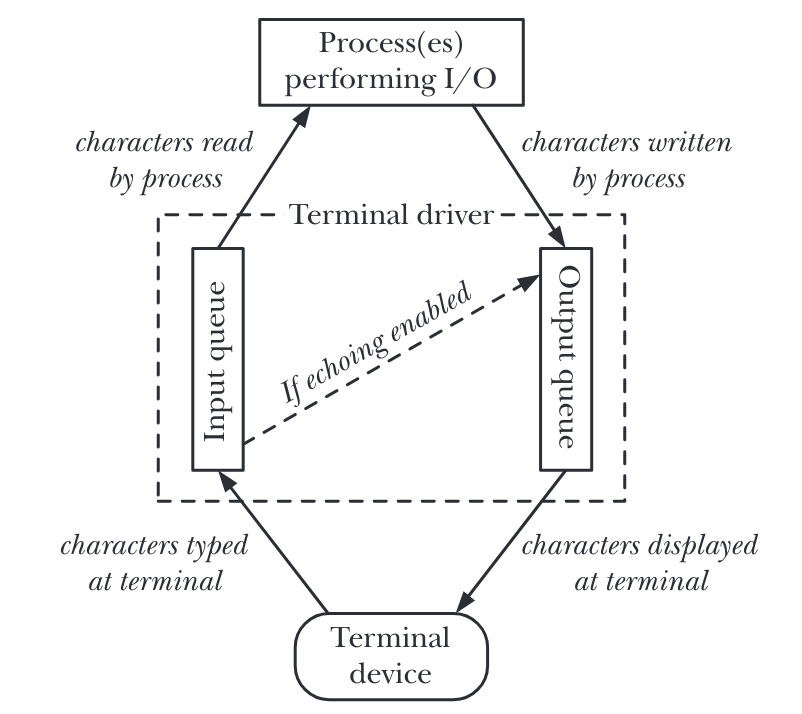
\includegraphics[width=250px, height=250px]{input_output_queue.png}
	\caption{Schéma montrant le tampon d'entrée et sortie dans le pilote de terminal}
\end{figure}


\chapter{Le pseudo-terminal}
Le pseudo-terminal, comme son nom l'indique, est un \textit{faux terminal}. Il joue un rôle crucial non seulement sous Linux, mais aussi sur les systèmes d'exploitation de type Unix tels que macOS, car il est utilisé par les émulateurs de terminal (comme \textit{Konsole} sur KDE) ainsi que par des programmes tels que \textit{ssh}.

\section{Le fonctionnement d'un pseudo-terminal}
Une paire de pseudo-terminaux est créée par le noyau. L'un joue le rôle de \textit{maître}, tandis que l'autre joue le rôle d'\textit{esclave}. Les deux paires communiquent entre elles de manière asynchrone, comme le ferait un \textit{pipe}. 

\begin{tcolorbox}[title=SystemV UNIX98 ou BSD]
La manière dont les pseudo-terminaux sont créés et utilisés varie selon le type d'API que le noyau utilise. Il existe ce qu'on appelle \textbf{UNIX98}, qui utilise deux répertoires spéciaux dans \textit{/dev}, à savoir \textit{/dev/ptmx} et \textit{/dev/pts/N}. L'autre s'appelle \textbf{BSD}, qui utilise le répertoire \textit{/dev/ptyXY} et \textit{/dev/ttyXY}. Cependant, le fonctionnement reste le même, que l'on utilise l'API System V \textit{UNIX 98} ou \textit{BSD}.
\end{tcolorbox}

Lorsqu'on lance l'émulateur de terminal en cliquant sur l'icône \textit{terminal ou console} sur le bureau, un processus est initié. Simultanément, le noyau crée une paire de pseudo-terminaux, établissant ainsi une connexion où l'un agit en tant que maître, lié à l'émulateur de terminal, et l'autre agit en tant qu'esclave, lié au processus lecteur, généralement un shell tel que Bash. Cette configuration permet une communication bidirectionnelle entre l'émulateur de terminal et le shell associé, assurant ainsi le fonctionnement fluide de l'environnement terminal.

Le processus lecteur est engendré par un appel à la fonction \textit{fork()} depuis le processus de l'émulateur de terminal. Afin d'éviter tout dysfonctionnement potentiel, il est impératif que le processus lecteur se détache de la session du processus parent. Cette séparation est cruciale pour garantir une exécution indépendante et stable. La section intitulée \textit{Le terminal de contrôle} aborde succinctement ce concept.

\section{Le terminal de contrôle}
Le terminal de contrôle est celui qui gère les entrées, sorties et \textit{jobs} d'une session. Sur Linux, on trouve ce qu'on appelle des \textit{groupes de processus} et des \textit{sessions}. Chaque session peut regrouper plusieurs groupes de processus, et à l'intérieur de chaque groupe, un ou plusieurs processus peuvent être en cours d'exécution. De plus, il existe un \textit{leader} par session et par groupe. Un processus peut occuper simultanément le rôle de leader de session et de leader de groupe.

Pour chaque session, il existe un seul \textit{terminal de contrôle} associé, et ce terminal de contrôle est désigné pour le groupe de processus que l'on appelle \textit{foreground} (en avant-plan), contrairement à d'autres groupes qui sont en \textit{background} (en arrière-plan). Seul un groupe de processus peut être en avant-plan, tandis que les autres groupes de processus sont en arrière-plan.

\begin{figure}[h]
        \centering
        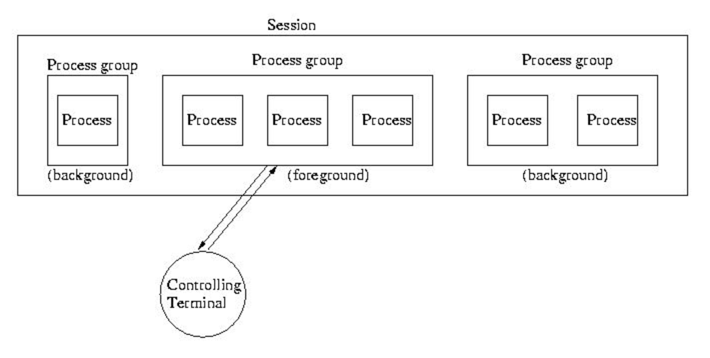
\includegraphics[width=200px, height=150px]{controlling_terminal.png}
        \caption{Schéma montrant un terminal de contrôle désigné pour un groupe de processus}
\end{figure}

Les \textit{jobs} sur Linux représentent des processus qui peuvent être de trois types principaux : \textit{avant-plan}, \textit{arrière-plan} et \textit{suspendu}. Lorsqu'un utilisateur exécute une commande dans le shell, un processus est créé pour exécuter cette commande. Si ce processus nécessite une interaction immédiate avec l'utilisateur, il est exécuté en \textit{avant-plan}, ce qui signifie que l'utilisateur doit attendre la fin de son exécution avant de pouvoir utiliser à nouveau le shell.

En revanche, si l'utilisateur souhaite libérer le shell pour d'autres commandes tout en laissant le processus s'exécuter en arrière-plan, il peut le démarrer en tant que \textit{job arrière-plan}. Cela permet à l'utilisateur de continuer à travailler dans le shell pendant que le processus s'exécute en tâche de fond.

Le type \textit{suspendu} se réfère à un \textit{job} qui a été temporairement stoppé, généralement par une combinaison de touches comme Ctrl-Z. Il peut ensuite être repris en arrière-plan ou en avant-plan.

\begin{tcolorbox}[title=Comment savoir quel est mon terminal de contrôle?]
Pour savoir quel terminal de contrôle est attaché au \textit{shell} en cours d'exécution, il suffit d'utiliser la commande : \textbf{tty}. Cette commande affichera le chemin absolu du terminal de contrôle qui \textit{contrôle} ce \textit{shell}. Si vous utilisez cette commande sur un émulateur de terminal, le terminal de contrôle sera le pseudo-terminal esclave rattaché au processus qui exécute le \textit{shell}. Dans le cas des consoles virtuelles (voir le chapitre concernant le terminal virtuel), il n'y a pas de notions de pseudo-terminaux. Le noyau simule un terminal physique directement et rattache ce terminal de contrôle à la console virtuelle.
\end{tcolorbox}

\begin{tcolorbox}[title=Utilisation de la commande sur l'émulateur de terminal]
\begin{verbatim}
user@localhost:~/Documents>tty
/dev/pts/2
user@localhost:~/Documents>_
\end{verbatim}
\end{tcolorbox}

\begin{tcolorbox}[title=Utilisation de la commande sur la console virtuelle]
\begin{verbatim}
user@localhost:~>
/dev/tty2
user@localhost:~>_
\end{verbatim}
\end{tcolorbox}

\section{Le programme pilote}
Avec tout ce bagage d'informations, nous connaissons plus ou moins les bases du fonctionnement des terminaux et pseudo-terminaux. Cependant, un problème subsiste : comment les entrées au clavier sont-elles interprétées par le maître ? \textit{Est-ce que c'est l'extrémité maître du pseudo-terminal qui récupère les entrées directement du clavier ?} La réponse est bien sûr que \textbf{non}.

Comme dit plus haut, l'émulateur de terminal est un processus qui tourne dans le système. Il possède son propre \textit{pid} et on peut même aller vérifier qui est son parent. Il n'y a pas de hasard sur Linux. Sachant que l'émulateur de terminal est directement rattaché à l'extrémité maître, c'est le seul processus qui peut être capable d'intercepter les données entrées sur le clavier.

Dans le livre de \textit{Michael Kerrisk} sur \textit{The Linux Programming Interface}, il fait référence à un programme pilote qui renvoie les entrées au clavier directement à l'extrémité maître, sans pour autant expliquer ce qu'est ce \textit{programme pilote}. Après plusieurs recherches, c'est le \textit{serveur d'affichage} sur Linux qui reçoit des \textit{events} de la part des pilotes (clavier, etc..). D'ailleurs une explication rapide avait été donné dans le chapitre \textit{Terminal virtuel} dans la section \textit{pilote de terminal}.

\hfill \break

Le serveur d'affichage (par exemple : X11) reçoit les \textit{events} et transmet l'information au programme qui tourne, dans notre cas, c'est l'émulateur de terminal. On s'aperçoit très vite que le \textit{programme pilote} dont Kerrisk parlait était en fait l'émulateur de terminal. Et ceci colle très bien, c'est bien l'émulateur de terminal qui envoie les données à l'extrémité maître et le maître renvoie les données en entrée à l'extrémité esclave.

\begin{figure}[h]
	\centering
	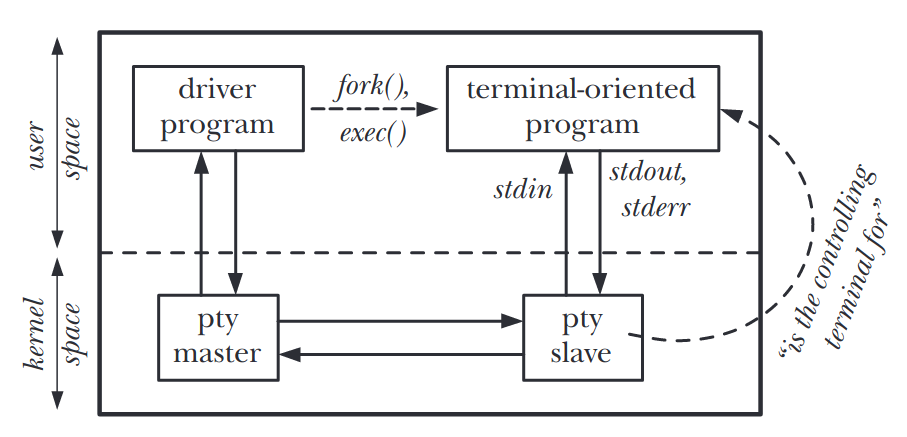
\includegraphics[width=200px, height=120px]{pseudo-terminal.png}
	\caption{Schéma montrant la communication entre 2 processus en utilisant le pseudo-terminal}
\end{figure}

Sur le schéma ci-dessus, les deux processus se distinguent : d'un côté, le \textit{programme pilote}, de l'autre, le \textit{bash}. On remarque l'inscription \textit{terminal-oriented program}, ce qui signifie simplement qu'il s'agit d'un programme ayant besoin de 'quelque chose' simulant un terminal. Et cette 'quelque chose' n'est autre que l'extrémité esclave, jouant le rôle de terminal de contrôle pour le programme. En quelque sorte, le programme 'pense' qu'il utilise un terminal.

\chapter{Mise en pratique}
Dans ce chapitre, j'utiliserai plusieurs appels système et implémenterai un petit programme en C afin d'observer de plus près le fonctionnement des pseudo-terminaux. Le but ici n'est en aucun cas de recréer quelque chose qui existe déjà. Autrement dit, je ne vais pas créer un pseudo-terminal et le manipuler, puisque je peux déjà utiliser les pseudo-terminaux directement créés par le noyau. Ainsi, les appels système tels que \texttt{posix\_openpty()}, \texttt{forkpty()}, etc., expliqués dans le livre de \textit{Michael Kerrisk}, ne seront pas utilisés. L'objectif concret est de 'fouiller' et voir comment tout fonctionne, tout en ayant un esprit critique à son égard.

\begin{tcolorbox}[title=Nota bene, colback=red!20]
Le programme implémenté ne fonctionnera pas sur le système d'exploitation Windows\texttrademark{}, car celui-ci n'utilise pas les pseudo-terminaux ou les utilise d'une autre manière. Concernant MacOS\texttrademark{}, celui-ci utilise bel et bien les pseudo-terminaux, mais d'une autre manière qui ressemble très fort au \textit{BSD-style} (voir chapitres précédents).
\end{tcolorbox}

\textcolor{red}{\textbf{Le programme a été testé et utilisé sur une distribution OpenSUSE (version 15.4) avec l'environnement de bureau KDE Plasma.}}

\vspace{\baselineskip}

Maintenant, le fonctionnement des pseudo-terminaux n'est plus un secret. Dans la très grosse majorité des distributions Linux, ce sont les pseudo-terminaux UNIX 98 qui sont utilisés, et c'est le noyau qui crée une nouvelle entrée dans le répertoire \textit{/dev/pts} lorsqu'il faut un pseudo-terminal. Ce programme va donc toujours utiliser les fichiers spéciaux qui se trouvent dans ce répertoire, d'où la petite mention \textit{Nota bene} au-dessus, entre autres.

\newpage

\section{Une lecture depuis le tampon d'entrée du pseudo-terminal esclave}
Est-ce que ce serait possible qu'on puisse lire depuis le tampon d'entrée d'un pseudo-terminal en cours d'utilisation sur le système ? On sait que le pseudo-terminal utilise deux tampons, un d'entrée et un autre de sortie. La réponse est \textbf{oui}.

Pour ce faire, il faut d'abord trouver où circulent les données, car on ne peut pas réellement accéder à ce tampon. Pour cela, un petit rappel concernant le terminal de contrôle. On avait vu que le terminal de contrôle gère les entrées, sorties et les \textit{jobs}. Le seul moyen de savoir quel est le terminal de contrôle du bash en cours d'utilisation, c'est d'utiliser la commande \textit{tty}. Une autre manière que je n'ai pas spécifiée, c'est aussi la commande \textit{ps aux} en regardant la colonne \textit{TTY}.

Une fois que le terminal de contrôle, qui est le pseudo-terminal esclave, est trouvé, il suffit d'effectuer une ouverture avec l'appel système \textit{open}, le but étant de récupérer le descripteur de fichier du pseudo-terminal esclave.

\begin{verbatim}
if( (fd = open(path, O_RDONLY)) < 0 ) {
                perror("open");
                exit(EXIT_FAILURE);
}
\end{verbatim}

Le \textit{path} est le chemin absolu vers le pseudo-terminal esclave (par exemple : /dev/pts/2). Ensuite, pour lire les entrées depuis le pseudo-terminal esclave, il faut utiliser l'appel système \textit{read}. Mais comme vu précédemment, le bash, qui est le \textit{programme lecteur}, ne lit les données de l'entrée uniquement si un caractère spécial qui joue le rôle de délimiteur est spécifié. C'est le caractère spécial \textbf{EOF} (ou \textbackslash n). Il faut à tout prix éviter un blocage inutile, puisque \textit{read()} va bloquer tant qu'il n'y a pas de données disponibles. Pour y remédier, on utilise l'appel système \textit{select}.

L'appel système \textit{select} permet d'effectuer une surveillance sur des descripteurs de fichiers et d'avertir lorsqu'un ou plusieurs descripteurs sont prêts pour la lecture ou l'écriture. Ces descripteurs de fichiers, \textit{select} les stocke dans des structures \textbf{fd\_set}.

Deux macros sont utilisées pour cela, \textit{FD\_ZERO}, qui permet de nettoyer la structure, et \textit{FD\_SET}, qui permet d'ajouter un descripteur de fichier dans une structure.

\newpage

\begin{verbatim}
FD_ZERO(&readfds);
FD_SET(fd, &readfds);

while( (select(fd + 1, &readfds, NULL, NULL, NULL)) 
				> 0 && strncmp("q", bytes, 1) != 0) {
	read(fd, bytes, 1);
        write(1, bytes, sizeof(bytes));
        FD_ZERO(&readfds);
        FD_SET(fd, &readfds);
}
\end{verbatim}

Après cela, l'appel système \textit{select()} retournera le nombre de descripteurs de fichiers qui ont changé de statut, que ce soit dans la structure des descripteurs de fichiers pour la lecture ou l'écriture. Pour information, \textit{select()} peut effectuer une surveillance sur des descripteurs de fichiers pour la lecture ou l'écriture, il y a donc 2 structures d'ensembles.

On peut distinguer que des données ne sont pas lues et ne s'affichent pas sur le pseudo-terminal cible, c'est tout à fait normal. Quand le programme va lire le tampon d'entrée du pseudo-terminal cible, il va vider le tampon et le pseudo-terminal cible n'affichera pas les données, mais certaines données peuvent être lues directement par le pseudo-terminal cible. Ce phénomène est dû au fait que quand le programme va lire l'entrée, lorsqu'une nouvelle donnée sera entrée au clavier, le pseudo-terminal cible aura le temps de la lire à son tour et le programme ne connaîtra pas son existence, vu que le pseudo-terminal cible a vidé le tampon et que le programme se trouve avec un tampon d'entrée vide.

\begin{figure}[h]
        \centering
	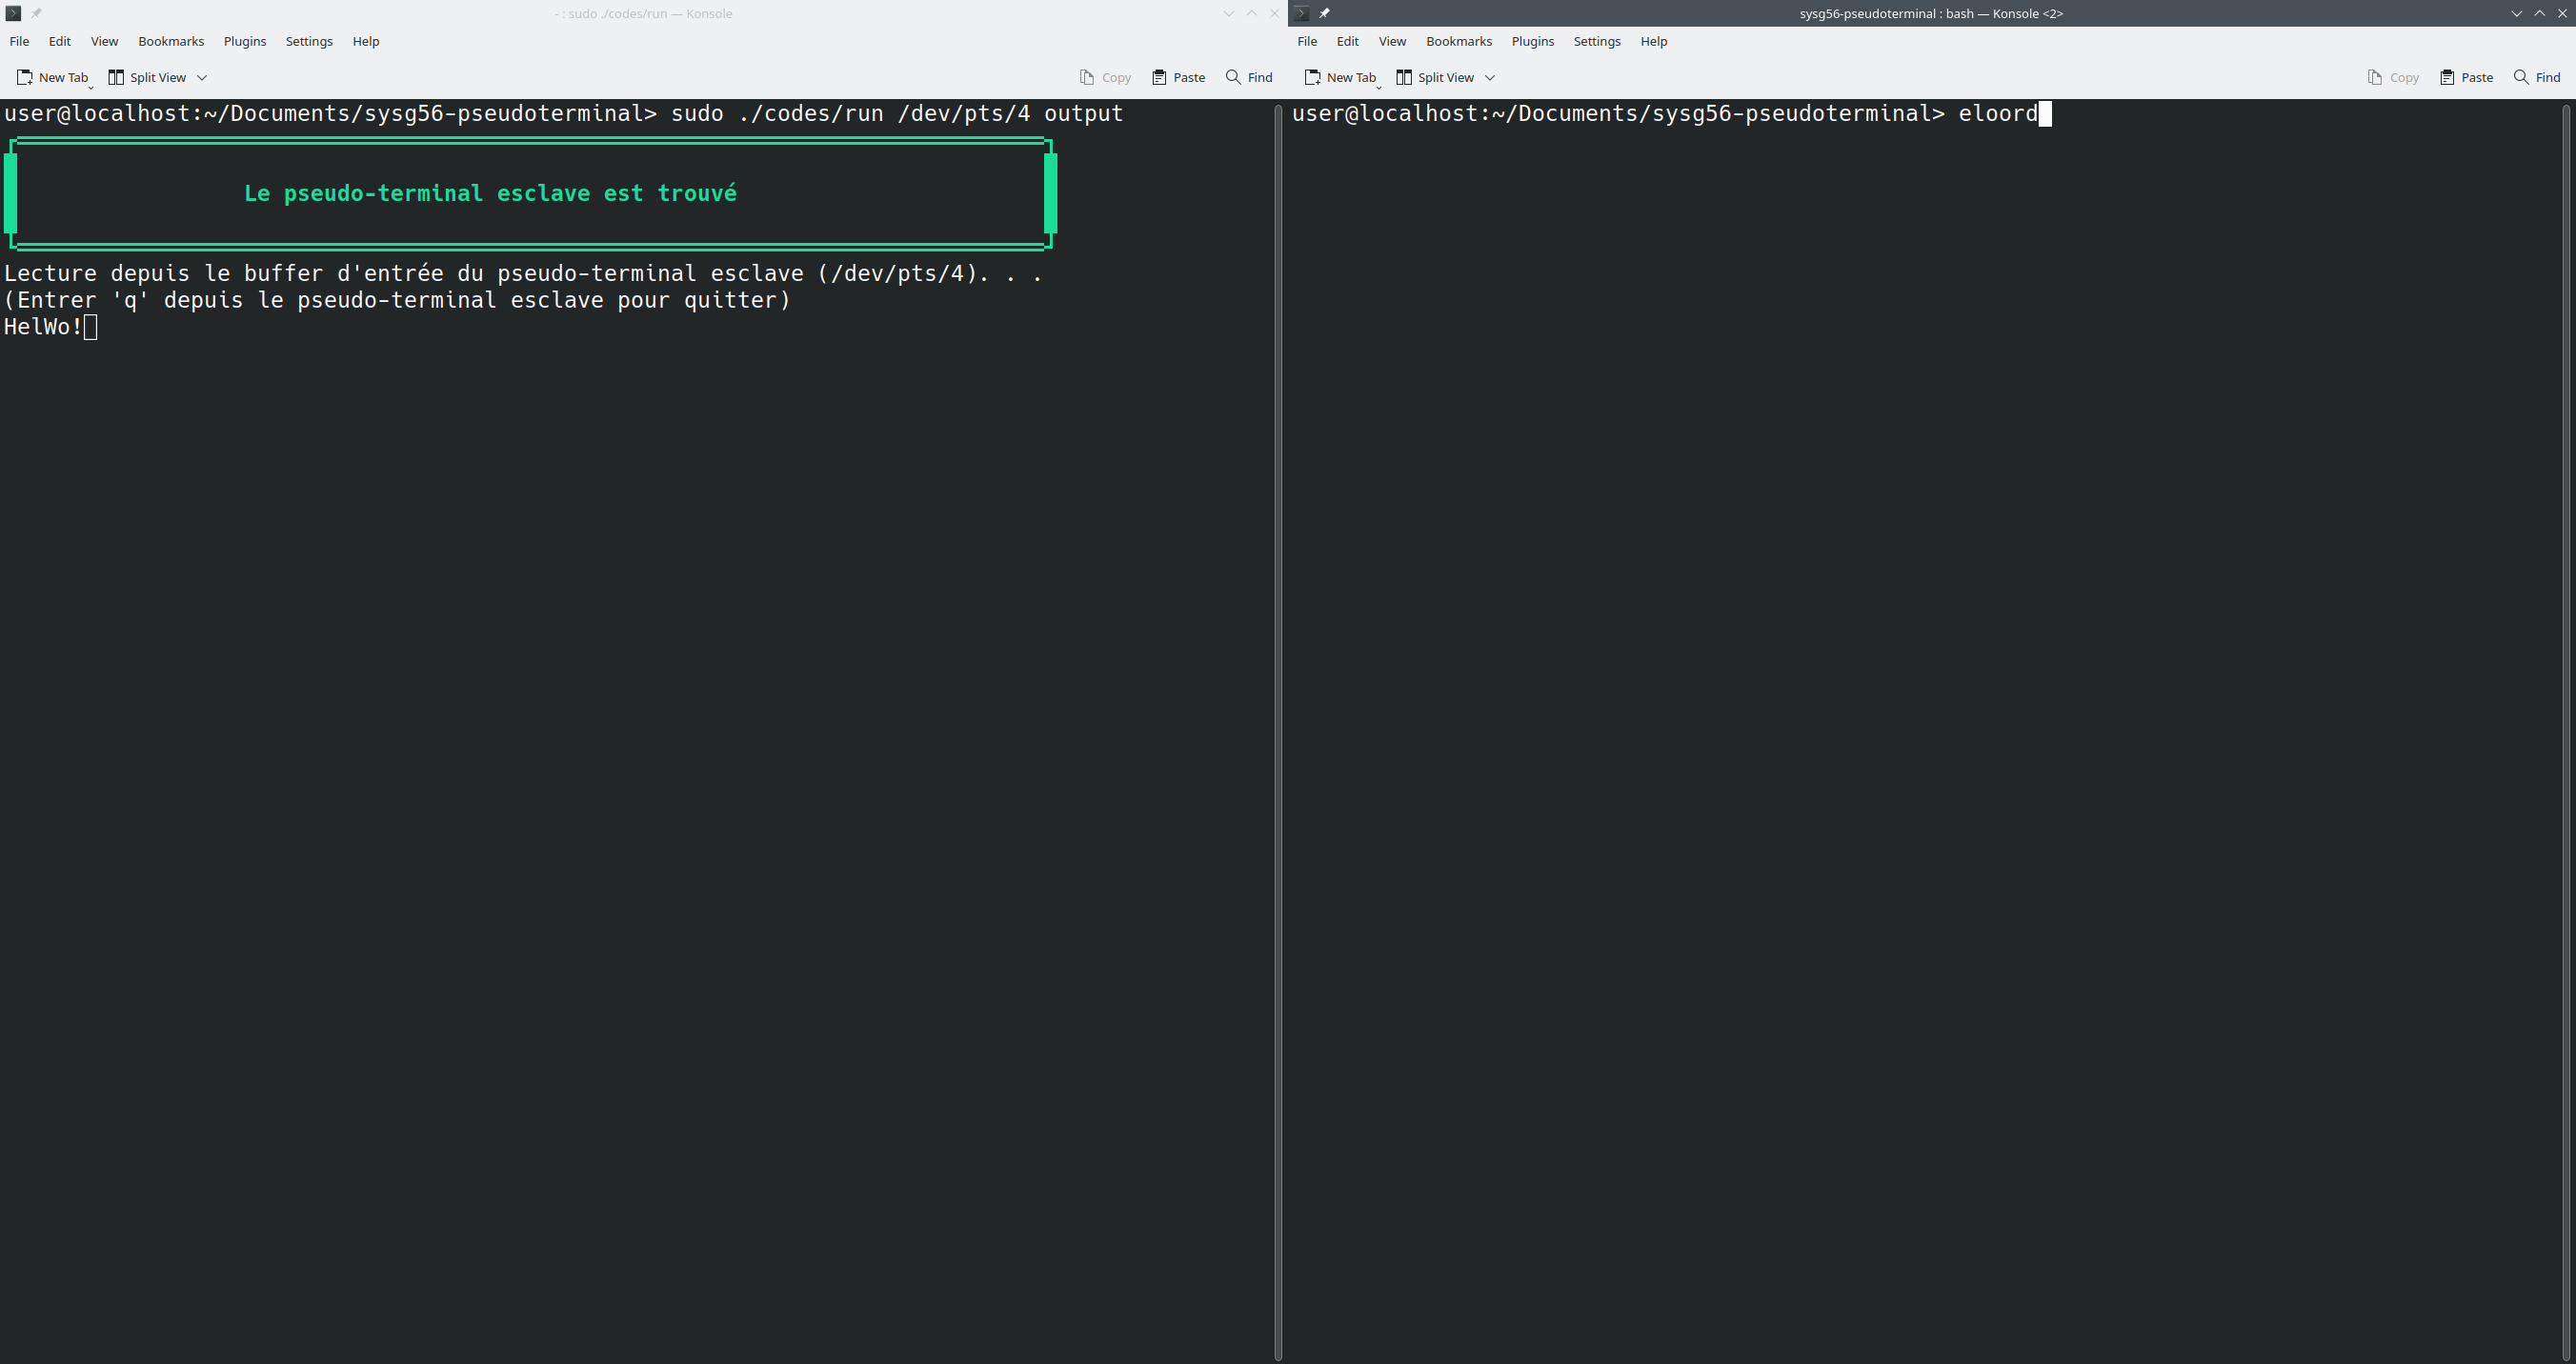
\includegraphics[width=250px, height=150px]{output.png}
	\caption{Exemple du programme (à gauche) qui lit l'entrée du pseudo-terminal esclave (à droite)}
\end{figure}

\section{Une écriture sur le tampon d'entrée du pseudo-terminal esclave}
Maintenant, on a vu que c'était possible de lire depuis le tampon d'entrée du pseudo-terminal esclave. Mais une autre étape à tester, c'est de voir si c'est possible d'écrire dans ce tampon. Sachant que le pseudo-terminal esclave fonctionne indépendamment de son côté en envoyant et recevant des données au maître, est-ce qu'un programme lambda peut directement altérer son fonctionnement et écrire dans ce tampon de telle sorte qu'une fois le pseudo-terminal esclave effectuera une lecture, il lira les données non pas reçues de la part du maître mais d'un programme extérieur.

Il est effectivement possible d'envoyer des données dans le tampon d'entrée du pseudo-terminal esclave. Il sera même possible de manipuler ce pseudo-terminal esclave comme si l'utilisateur interagissait directement avec lui. Bien sûr, que ce soit écrire ou lire (section précédente), il faut les droits root pour pouvoir utiliser le programme (et heureusement).

Pour ce faire, comme pour la section précédente pour la lecture, il faut d'abord ouvrir le pseudo-terminal esclave et récupérer son descripteur de fichier. Par la suite, il sera possible d'envoyer des données avec l'utilisation d'un appel système bien spécifique.

\begin{verbatim}
FD_ZERO(&writefds);
FD_SET(fd, &writefds);

while( (select(fd + 1, NULL, &writefds, NULL, NULL)) > 0 
                && ((messg = getchar()) != 'q') ) {
        if(ioctl(fd, TIOCSTI, &messg)) {
                        perror("ioctl");
                        exit(EXIT_FAILURE);
         }

FD_ZERO(&writefds);
FD_SET(fd, &writefds);
        }
\end{verbatim}

L'appel système en question est \textit{ioctl()}, qui permet de manipuler les paramètres d'un fichier spécial sous Linux. Petit rappel, dans les chapitres précédents, j'avais expliqué que le répertoire \textit{/dev} était un répertoire contenant des fichiers spéciaux. Et que ces fichiers étaient de types \textit{caractère} ou \textit{bloc}. Et l'appel système \textit{ioctl()} permet de manipuler ces fichiers spéciaux de type \textit{caractère}. Ça tombe bien, les pseudo-terminaux sont des fichiers spéciaux de types caractère.

\textit{man} est spécialement dédié aux pseudo-terminaux (\textit{man ioctl\_tty}). On peut y voir plusieurs commandes différentes qui permettent d'effectuer des opérations précises. La commande qui nous intéresse, c'est \textbf{TIOCSTI}.

\newpage

Une fois que les données seront stockées dans la variable \textit{messg} et que \textit{select()} avertira qu'une écriture est autorisée sur le pseudo-terminal esclave, l'appel système va envoyer les données stockées dans \textit{messg} dans le tampon d'entrée du pseudo-terminal esclave.

\begin{figure}[h]
        \centering
        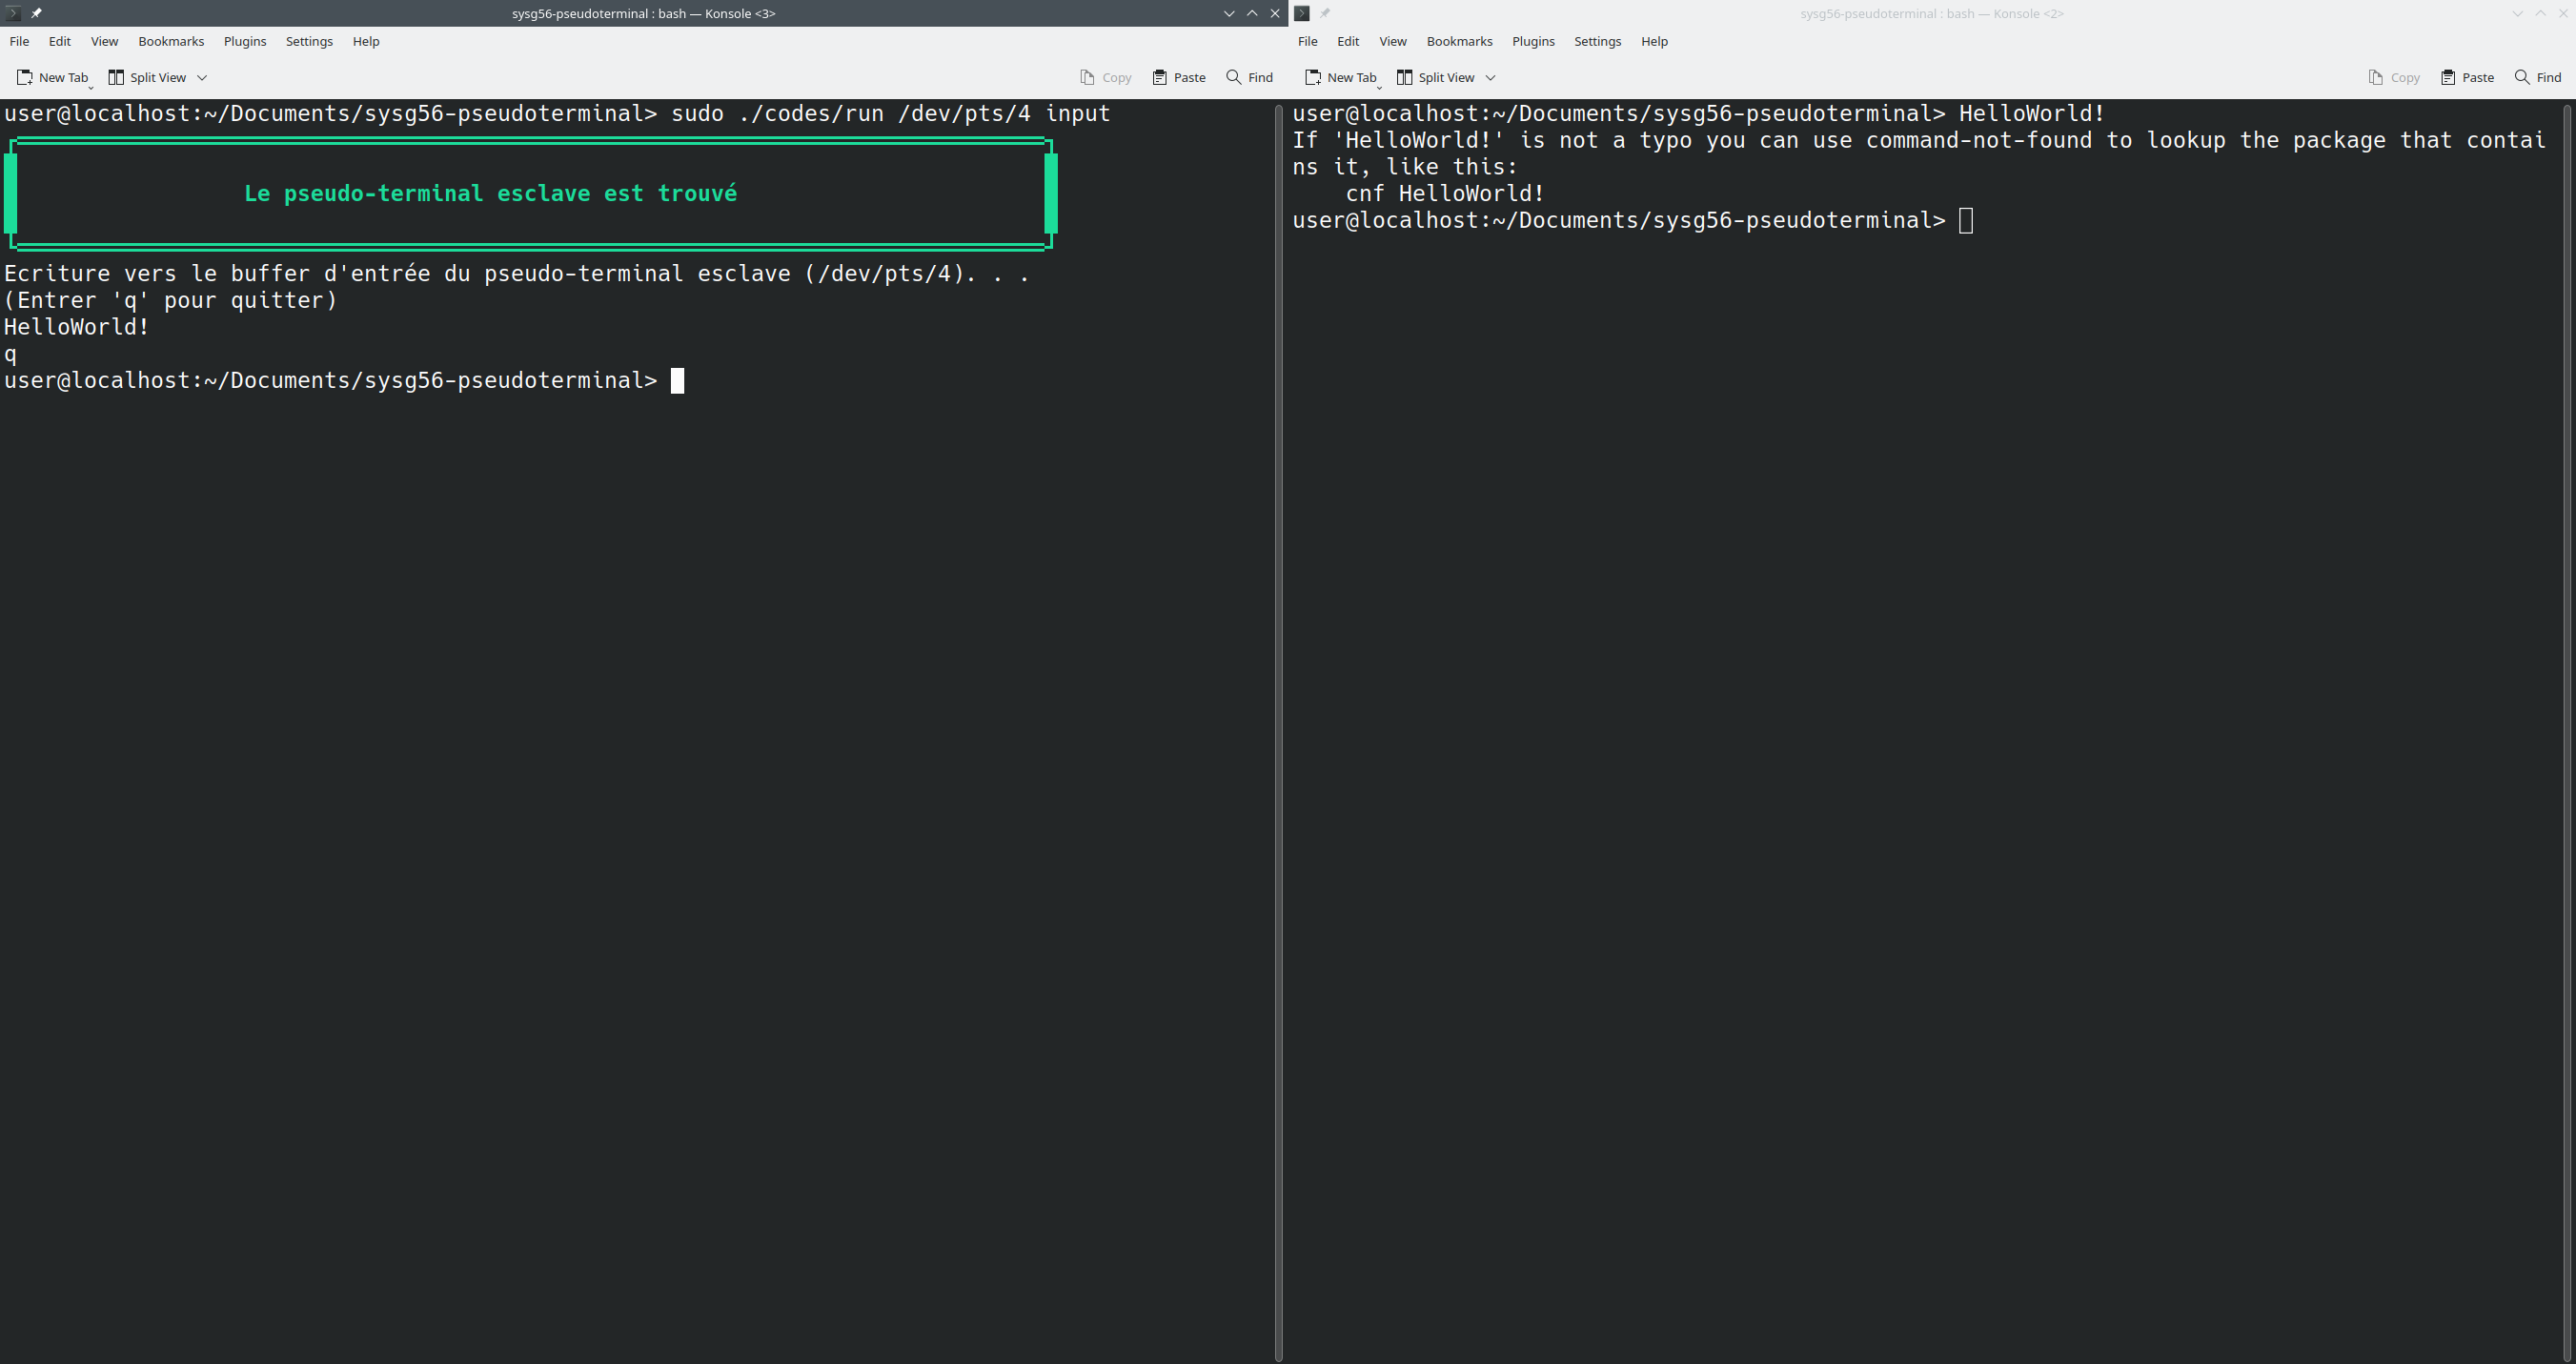
\includegraphics[width=250px, height=150px]{input.png}
        \caption{Exemple du programme (à gauche) qui écrit dans l'entrée du pseudo-terminal esclave (à droite)}
\end{figure}

\begin{tcolorbox}[title=Pour information]
	L'appel système \textit{ioctl} est très puissant. Il est aussi possible d'obtenir des informations à propos d'un pseudo-terminal, de récupérer la taille de la fenêtre du pseudo-terminal (en réalité, c'est la taille de la fenêtre de l'émulateur de terminal), de détacher le terminal de contrôle d'un processus et plein d'autres commandes très utiles...
\end{tcolorbox}


% ==========================

\nocite{*} % Ignorer citations et afficher les données du fichier references.bib
\bibliographystyle{plain}
\bibliography{references}
\end{document}
